\documentclass[aspectratio=169,10pt]{ctexbeamer}

% =========================
% 主题与样式
% =========================
\usetheme{Madrid}
\usecolortheme{dolphin}
\setbeamertemplate{navigation symbols}{}
\setbeamertemplate{footline}[frame number]

% =========================
% 常用宏包
% =========================
\usepackage{graphicx}
\usepackage{booktabs}
\usepackage{amsmath}
\usepackage{adjustbox}
\usepackage{makecell}
\usepackage{multirow}
\usepackage{hyperref}
\hypersetup{hidelinks}

% =========================
% 参考文献（直接复用 report.tex 的 biblatex + biber 流程）
% 编译顺序：XeLaTeX -> Biber -> XeLaTeX -> XeLaTeX
% =========================
\usepackage[
  backend=biber,
  style=references/gb7714-2015, % 文末参考文献：编号体例
  citestyle=authoryear,         % 文内引用：作者—年份体例
  gbnamefmt=none,
  gbpub=false,
  giveninits=true,
  uniquename=init,
  seconds=true,
  sorting=nyt,
  maxcitenames=1,
  mincitenames=1,
  maxbibnames=99,
  natbib=true,
  sortcites=false
]{biblatex}
\addbibresource{references/reference.bib}
\DeclareDelimFormat{nameyeardelim}{，}%
\DeclareDelimFormat{multicitedelim}{；}%
\renewcommand*{\mkbibparens}[1]{（#1）}

% 图片路径（优先使用 Writing 根目录下的英文文件名副本，避免路径/中文目录导致的编译问题）
\graphicspath{{./}}

% =========================
% 标题信息（来自 report.tex 封面）
% =========================
\title[关税冲击与城中村犯罪]{美国关税冲击对中国城中村的犯罪影响\\——来自珠三角的网格级别证据}
\author[花野]{花野}
\institute[经济学院]{经济学院}
\date{\today}

\begin{document}

% =========================
% 封面
% =========================
\begin{frame}[plain]
  \titlepage
\end{frame}

% =========================
% 目录
% =========================
\begin{frame}{汇报结构}
  \tableofcontents
\end{frame}

\section{研究背景}

\begin{frame}{研究背景：全球化退潮与贸易摩擦}
  \begin{itemize}
    \item 近年来\textbf{贸易保护主义与民粹主义抬头}，单边加征关税、设置贸易壁垒等行为日益频繁。
    \item 2004--2018 年间，美国长期是中国\textbf{第一大贸易伙伴/最大出口对象}之一，对美出口占中国出口总额一度接近\textbf{20\%}。
  \end{itemize}
  \vspace{0.4em}
  \begin{block}{核心关切}
    宏观贸易冲击除了经济后果，还可能通过就业与收入渠道转化为\textbf{城市治理与公共安全的社会成本}。
  \end{block}
\end{frame}

\begin{frame}{研究背景：2018 年对华加征关税冲击}
  \begin{itemize}
    \item 2018 年下半年，美国分三批对华加征关税：List 1/2 税率 25\%，List 3 起初 10\%（后续上调至 25\%）。
    \item 双边贸易平均关税由贸易战前约\textbf{3.1\%}上升至约\textbf{12.0\%以上}\citep{bown2021trade}。
    \item 2019 年中国对美出口总额较上年减少\textbf{597 亿美元}，美国从中国第一大贸易伙伴降为第二大（位居东盟之后）。
  \end{itemize}
\end{frame}

\begin{frame}{研究问题与核心发现}
  \begin{enumerate}
    \item \textbf{问题：}关税冲击是否推高城中村网格犯罪强度？正规与非正规街区之间有何差异？
    \item \textbf{落点：}同为城中村，新增的社会治理成本是集中在内城还是被逼退至城市外围？
  \end{enumerate}
  \vspace{0.6em}
  \textbf{主要发现：}
  \begin{itemize}
    \item 关税暴露度提高 1 个标准差，\textbf{城中村犯罪强度上升约 20.6\%}，正规街区无明显波动；
    \item 冲击带来的治安恶化具有不平衡性，\textbf{主要由城市外围城中村承载}；
    \item 类型上更多表现为\textbf{财产型（经济驱动）、冲动型及地下经济犯罪}的增幅更大。
  \end{itemize}
\end{frame}

\section{本文在文献生态中的位置}

\begin{frame}{已有文献与本文的切入点}
  \begin{itemize}
    \item 已有文献广泛讨论贸易冲击带来的\textbf{企业利润、就业与创新}等经济后果\citep{amiti2019impact,fajgelbaum2020return,ma2025market}。
    \item 对\textbf{社会后果}（如治安）讨论相对有限，仅少数工作（如 \citeauthor{ma2025market}\citeyearpar{ma2025market}）在更宏观尺度上提供相关证据。
    \item 笔者未能检索到\textbf{直接研究“关税冲击 $\rightarrow$ 犯罪”}的论文，尤其缺乏面向城市内部微观空间的识别。
  \end{itemize}
\end{frame}

\begin{frame}{为何需要更“细”的数据：数据限制与本文突破}
  \begin{itemize}
    \item 受数据限制，关注犯罪结果的研究多在\textbf{省级}，少部分前沿文献做到\textbf{市级/县级}，且多为\textbf{年度}数据，难以体现城市内部微观空间的异质性承载。
    \item 本文利用大语言模型从\textbf{22 万余份刑事裁判文书}抽取案发时间/地点/案由并进行地理编码，构建\textbf{100m 半年度网格面板}。
    \item 同时结合基于卫星数据识别的\textbf{城中村边界/占比}，实现正规与非正规街区、内城与外围的精细划分。
  \end{itemize}
  \vspace{0.4em}
  \begin{block}{本文贡献}
    将贸易摩擦的社会成本刻画从“城市平均效应”推进到\textbf{城市内部微观空间}。
  \end{block}
\end{frame}

\section{数据与变量}

\begin{frame}{数据：从裁判文书到100米网格面板}
  \begin{itemize}
    \item 样本：2015--2021年珠三角九市刑事一审判决书（约22万份）。
    \item 关键信息抽取：使用大语言模型从“经审理查明”段落提取
      \begin{itemize}
        \item 案发时间（归并至半年度）
        \item 案发地点（百度地图地理编码转经纬度）
        \item 案由（归并为16类/4大类）
      \end{itemize}
    \item 构造：点事件汇总到\textbf{100m规则网格}，得到半年度面板的犯罪计数（大量零值）。
  \end{itemize}
\end{frame}

\begin{frame}[plain,t]{数据概览：人口空间分布（2015--2020）}
  \begin{center}
    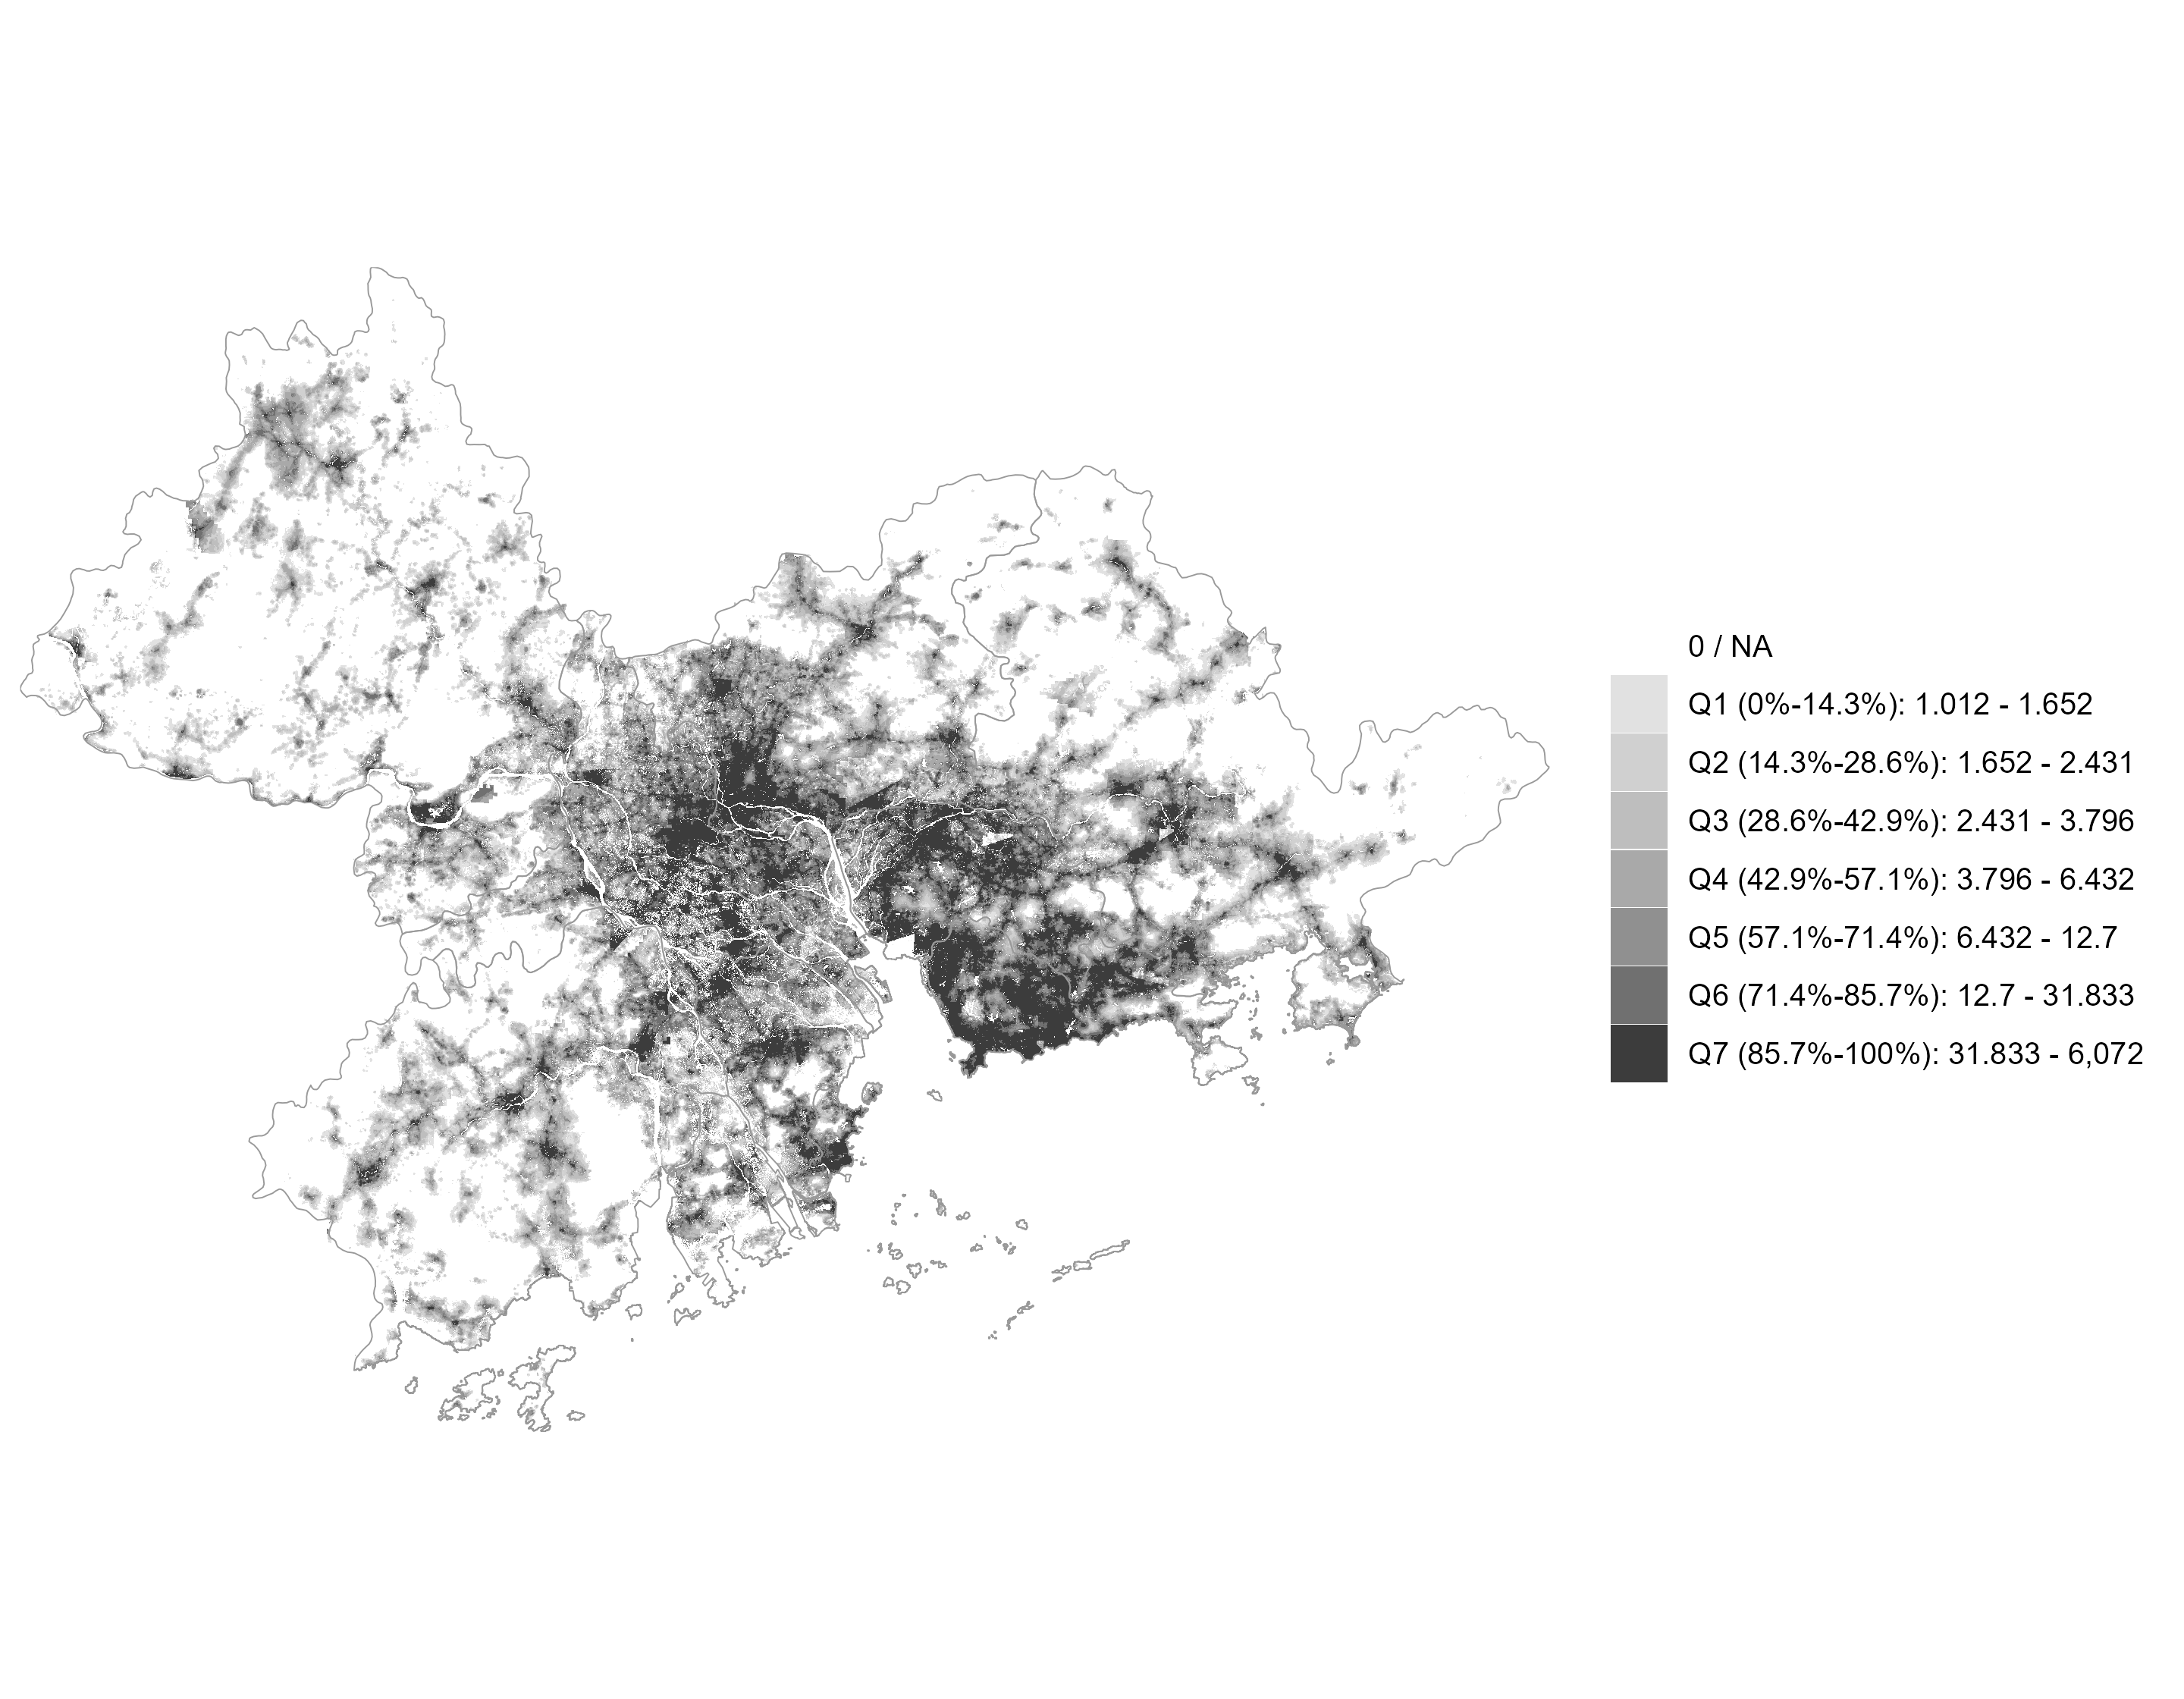
\includegraphics[width=0.70\textwidth]{1.描述性证据/分布图/prd_prefer500m_pop.png}
  \end{center}
  \vspace{-0.2em}
\end{frame}

\begin{frame}[plain,t]{空间对象：城中村网格识别与划分}
  \small 城中村识别来自Sentinel-2 + 深度学习结果，以“城中村面积占比 $>0$”定义100m城中村网格，并进一步区分城区内与城市外围。
  \vspace{0.4em}
  \begin{center}
    \includegraphics[width=0.68\textwidth]{urban_shape.png}
  \end{center}
\end{frame}

\begin{frame}[plain,t]{城中村空间形态与100米网格尺度示意}
  \begin{center}
    \IfFileExists{UV_shape.png}{\includegraphics[width=0.92\textwidth]{UV_shape.png}}{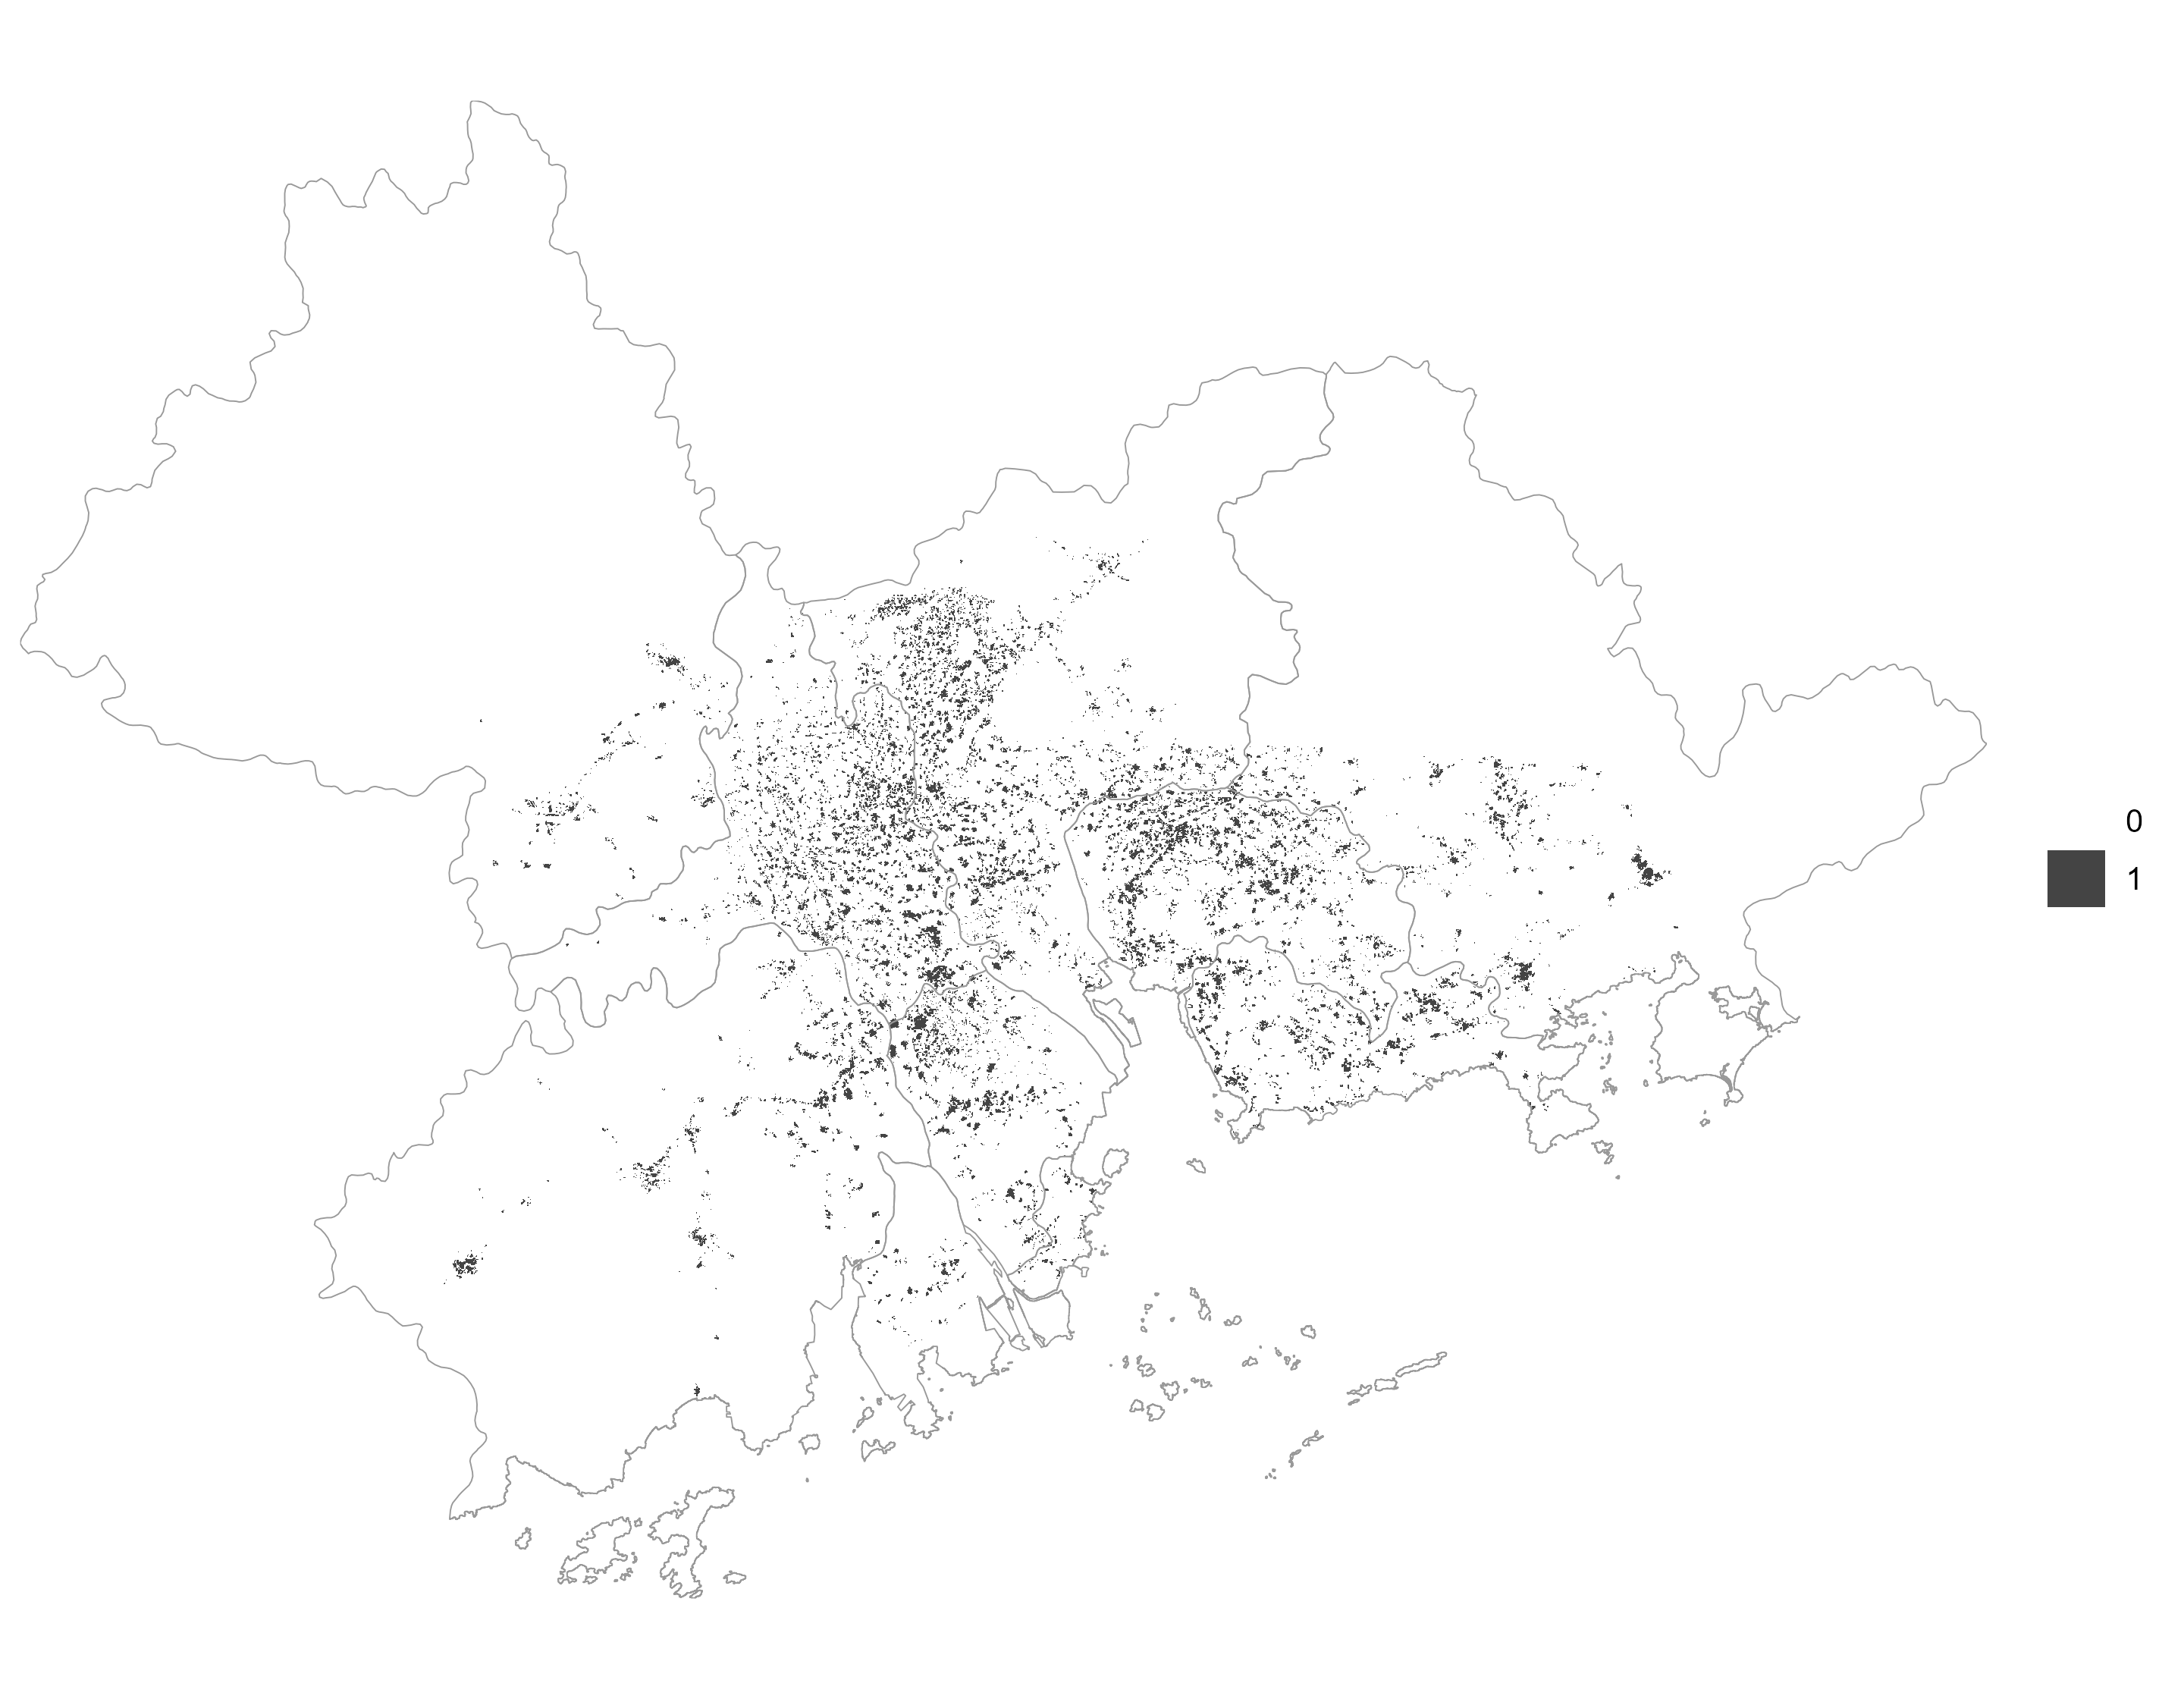
\includegraphics[width=0.92\textwidth]{1.描述性证据/分布图/prd_prefer500m_urban_village.png}}
  \end{center}
  \vspace{-0.2em}
  \small 红色网格为城中村栅格（颜色越深表示城中村面积占比越高）；本文基准空间尺度为100m。
\end{frame}

\begin{frame}[plain,t]{描述性证据：犯罪空间分布（2015--2020）}
  \begin{center}
    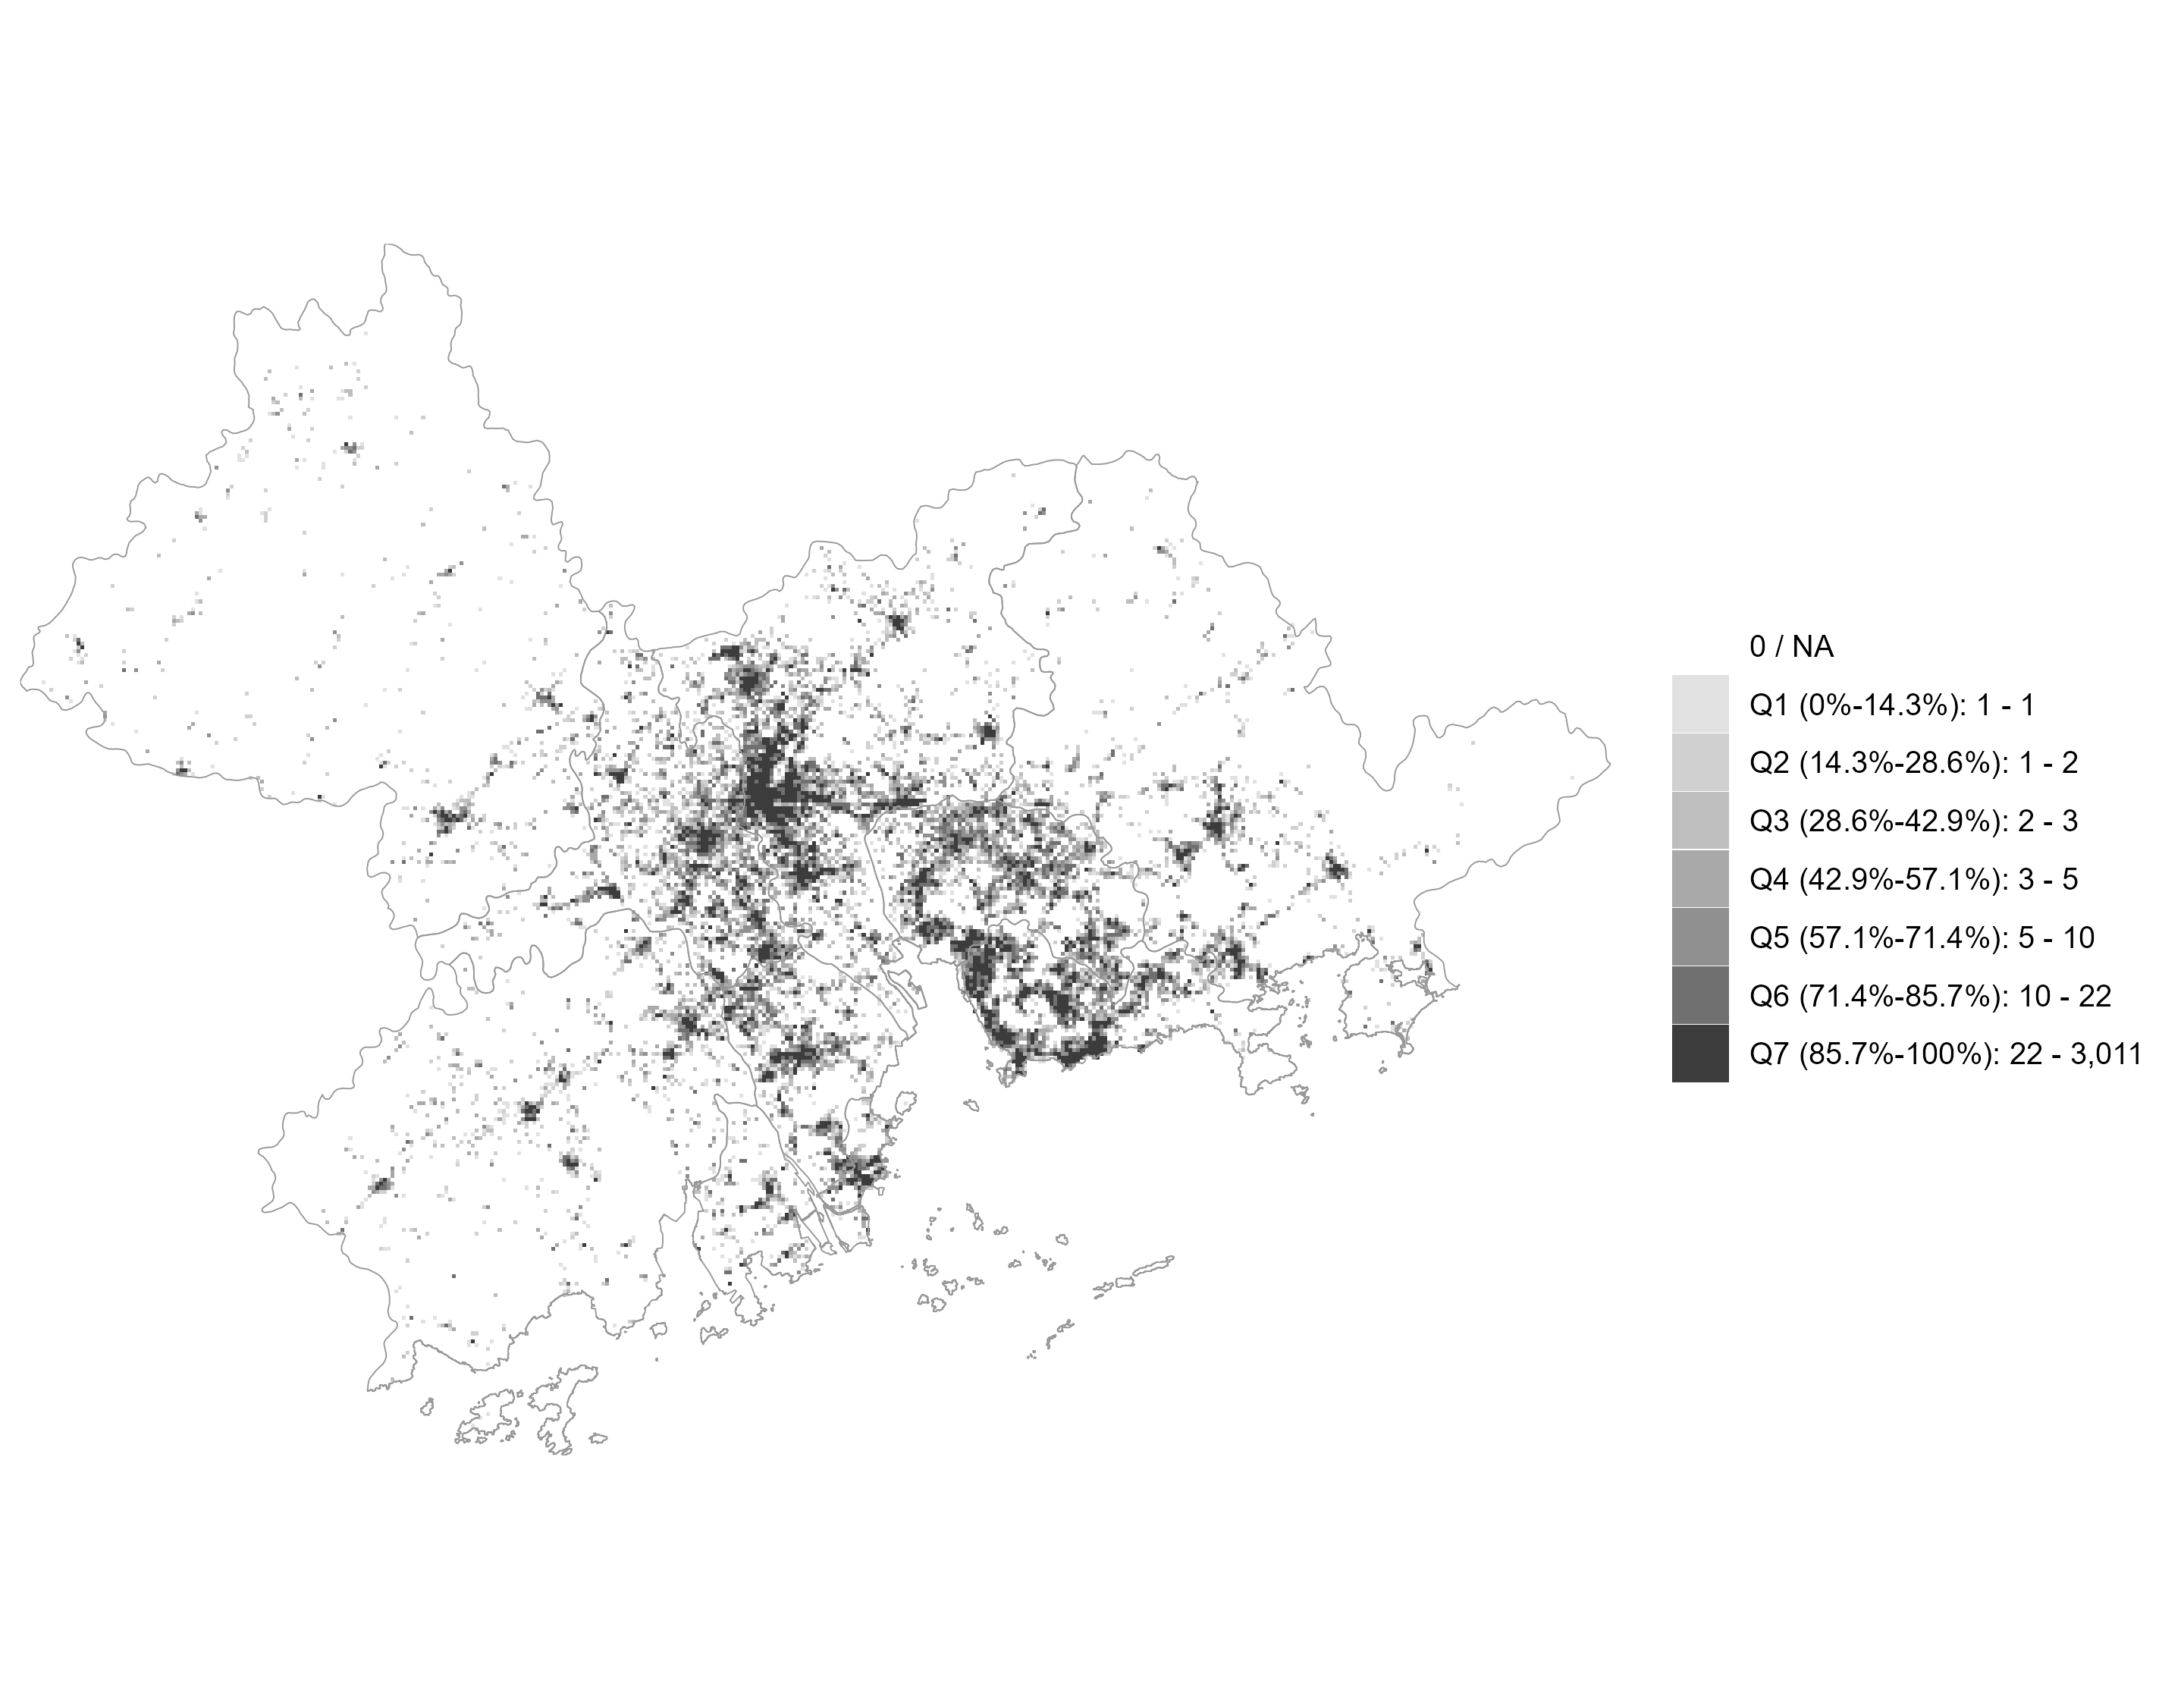
\includegraphics[width=0.70\textwidth]{prd_prefer500m_crime_count_1km.png}
  \end{center}
  \vspace{-0.2em}
\end{frame}

\begin{frame}{描述性统计：基线特征比较（表1）}
  \centering
  \scriptsize
  \begin{adjustbox}{width=\textwidth,center}
  \begin{tabular}{lccccc}
    \toprule
    变量 & 全样本 & 正规街区 & 城中村 & 中心城中村 & 外围城中村 \\
    \midrule
    关税暴露度 & \makecell{0.029\\(0.016)} & \makecell{0.024\\(0.008)} & \makecell{0.025\\(0.010)} & \makecell{0.025\\(0.008)} & \makecell{0.027\\(0.012)} \\
    人口密度 & \makecell{19.102\\(50.674)} & \makecell{54.356\\(94.380)} & \makecell{59.189\\(79.283)} & \makecell{72.760\\(90.596)} & \makecell{35.393\\(45.023)} \\
    十万人犯罪率 & \makecell{15.782\\(1520.161)} & \makecell{30.401\\(1999.833)} & \makecell{59.259\\(2695.463)} & \makecell{59.130\\(1358.386)} & \makecell{59.486\\(4094.982)} \\
    到公交车站距离 & \makecell{21854.506\\(25800.034)} & \makecell{5198.428\\(4806.057)} & \makecell{7134.018\\(7176.148)} & \makecell{5625.248\\(5146.584)} & \makecell{9779.328\\(9184.640)} \\
    到小学距离 & \makecell{1897.568\\(1709.585)} & \makecell{1201.118\\(774.719)} & \makecell{811.575\\(654.294)} & \makecell{723.624\\(559.138)} & \makecell{965.778\\(770.198)} \\
    到三甲医院距离 & \makecell{11049.707\\(10904.109)} & \makecell{3440.906\\(2202.143)} & \makecell{4193.076\\(4546.859)} & \makecell{2985.484\\(2118.458)} & \makecell{6310.334\\(6481.760)} \\
    到股份制商业银行距离 & \makecell{18566.608\\(24166.442)} & \makecell{2909.621\\(2315.000)} & \makecell{4196.608\\(5095.410)} & \makecell{2482.858\\(2078.694)} & \makecell{7201.306\\(7052.006)} \\
    网格数 & 2741736 & 487216 & 156741 & 99823 & 56918 \\
    样本期数 & 12 & 12 & 12 & 12 & 12 \\
    \bottomrule
  \end{tabular}
  \end{adjustbox}
  \vspace{0.35em}
  \parbox{0.95\textwidth}{\footnotesize 注：表中为政策实施前基线统计量的均值，括号内为标准差。}
\end{frame}

\begin{frame}[plain,t]{处理强度：县（区）关税暴露度（shift-share）}
  \small 以2016年对美出口结构作为事前份额，将产品层面的关税增量映射为县（区）暴露度；基准政策后期定义为\textbf{2018H2及之后}。
  \vspace{-0.25em}
  \begin{equation*}
    TariffExposure_{c,2018}=\sum_i \frac{Export_{c,i,2016}}{TotalExport_{c,2016}}\times \Delta \tau_{i,2018}.
  \end{equation*}
  \begin{center}
    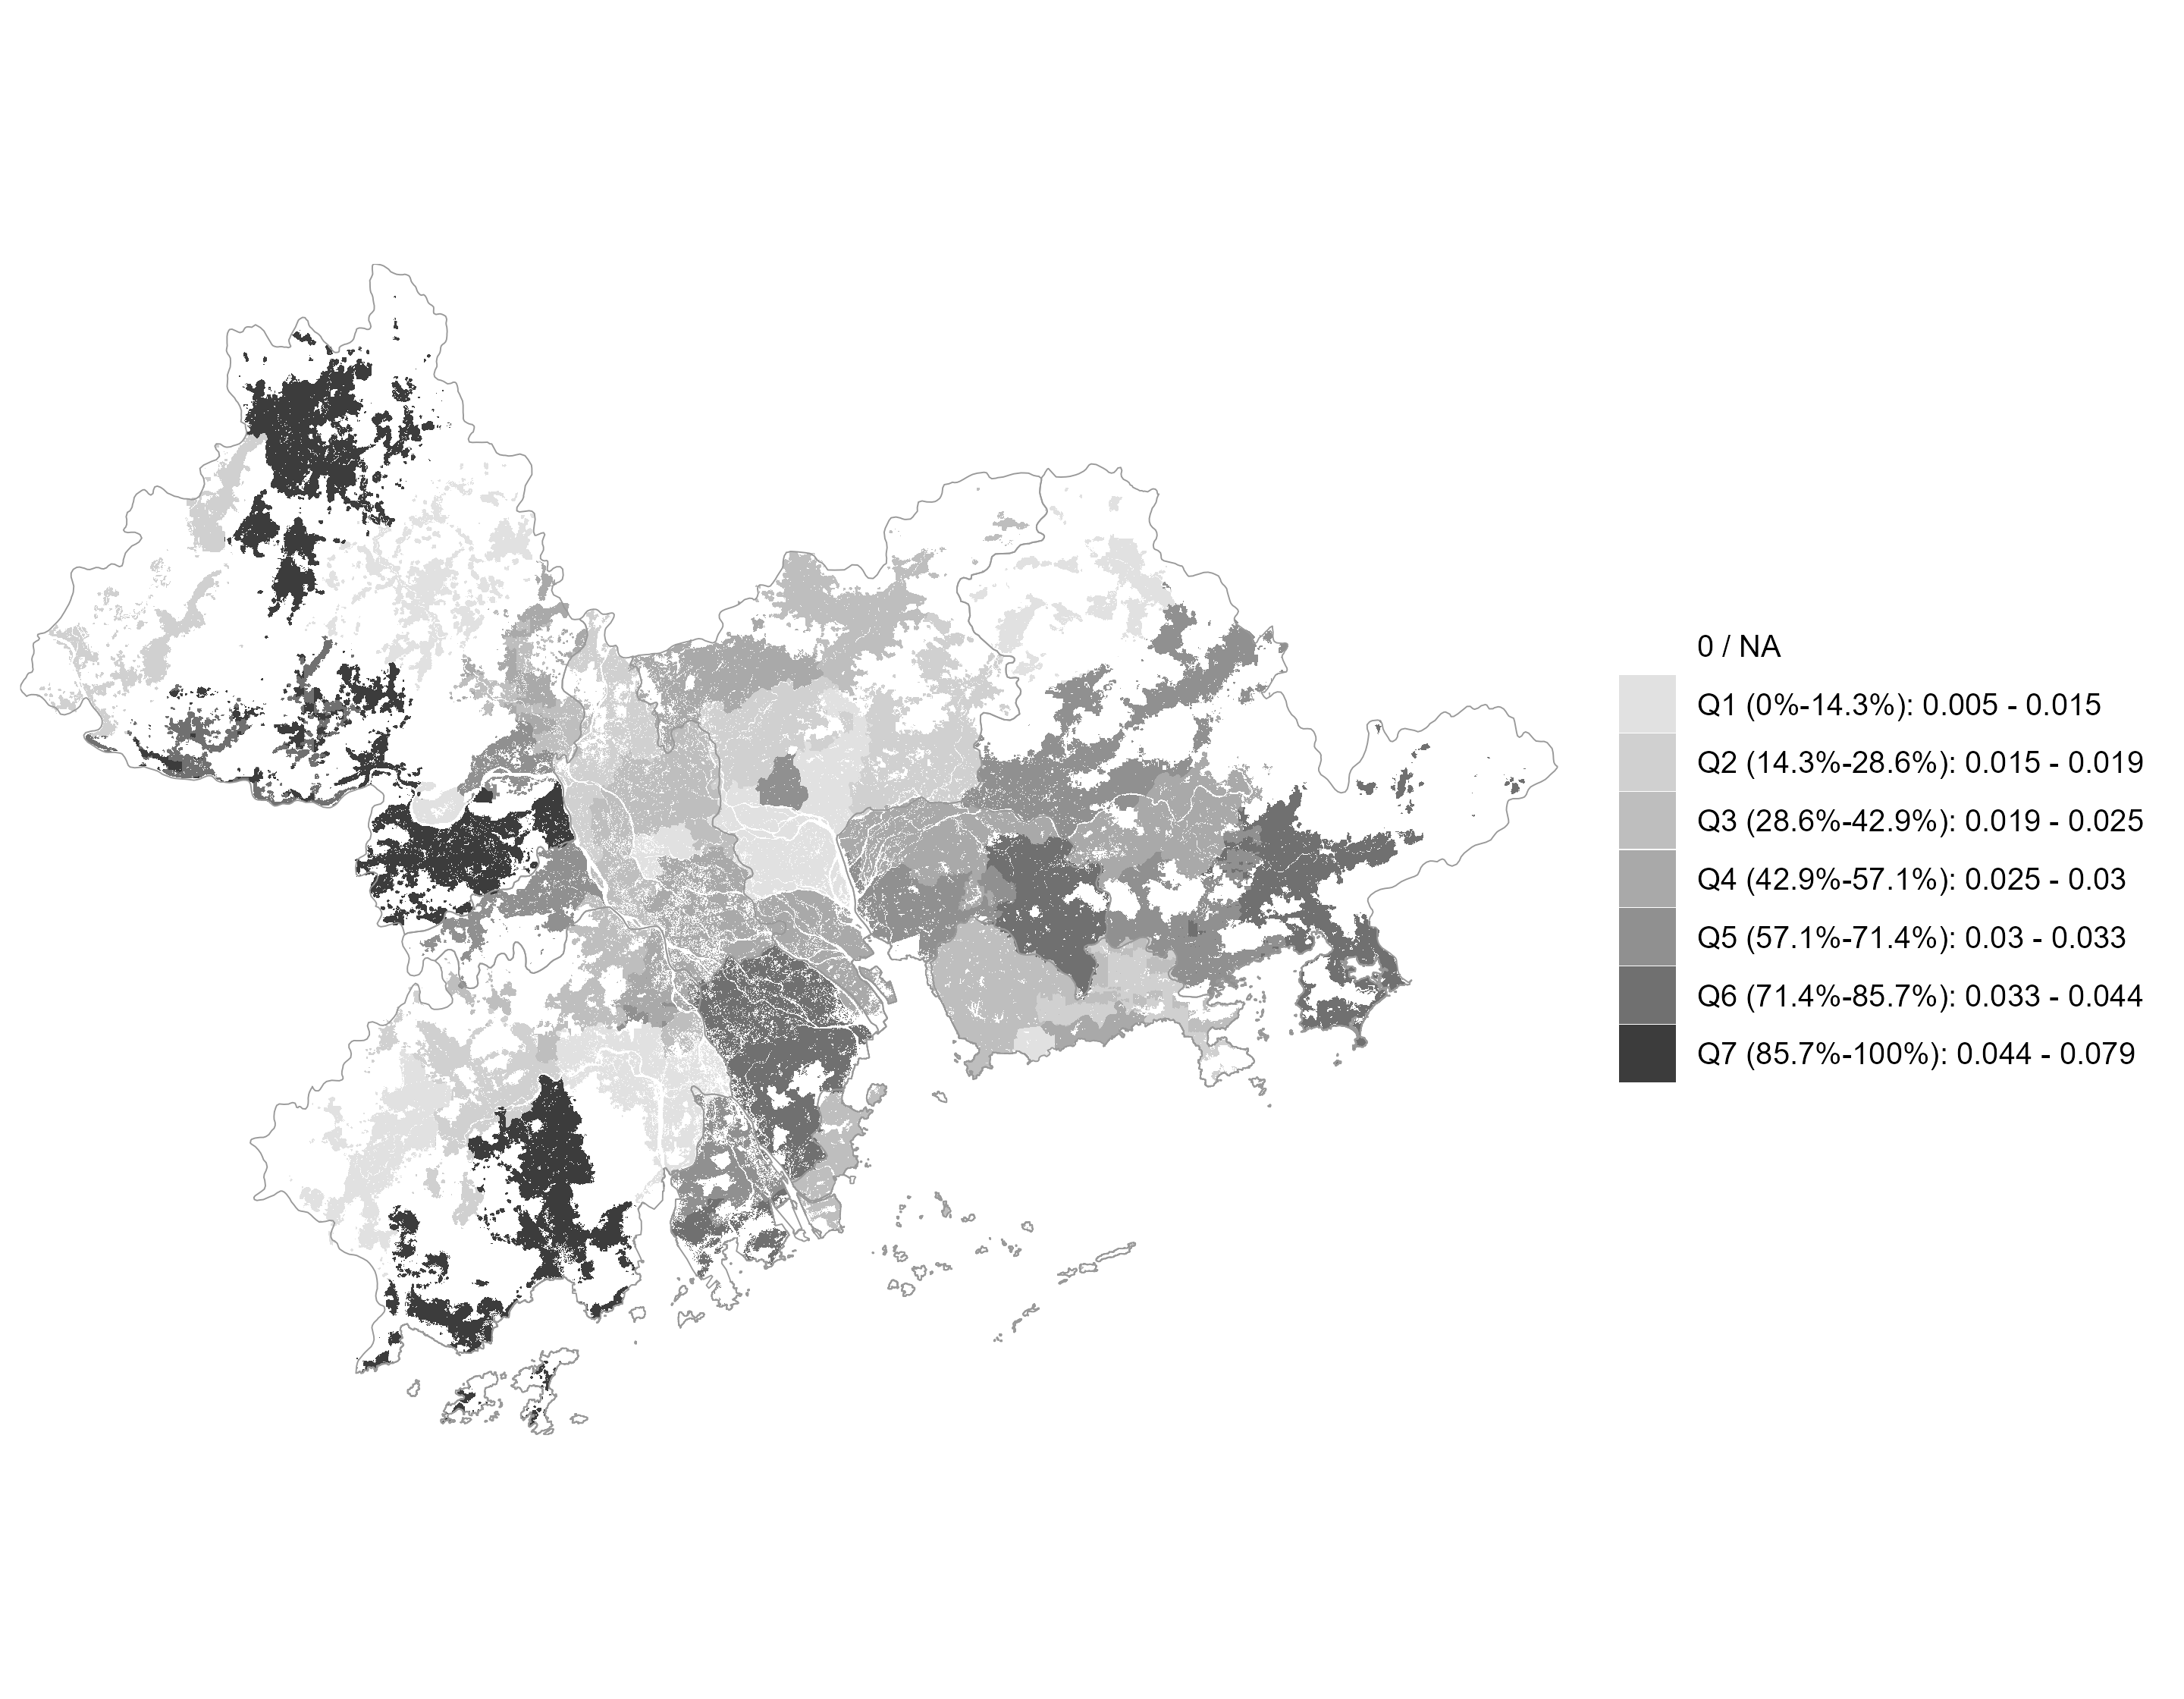
\includegraphics[width=0.58\textwidth]{1.描述性证据/分布图/prd_prefer500m_us_tariff_exposure_4.png}
  \end{center}
\end{frame}

\section{识别策略与基准结果}

\begin{frame}{识别策略：PPML连续DID（网格固定效应）}
  \begin{itemize}
    \item 因变量：网格半年度犯罪计数（非负整数、零值多）。
    \item 估计方法：PPML（避免 $\ln(0)$，对异方差稳健），加入人口offset控制规模差异。
    \item 固定效应：网格固定效应 + 城市$\times$半年度固定效应；标准误按县（区）聚类。
  \end{itemize}
  \vspace{-0.2em}
  \begin{equation*}
  \mathbb{E}[Crime_{g,c,t}\mid X]
  =\exp\Big(\beta\cdot Post_t\times Exposure_c+\delta_g+\gamma_{city,t}+\ln(Pop_{g,t})\Big).
  \end{equation*}
\end{frame}

\begin{frame}{基准结果：关税冲击显著推升城中村犯罪}
  \begin{itemize}
    \item 估计结果（城中村样本）：$Post\times Exposure$ 系数约为 0.188（1\%显著）。
    \item 经济含义：暴露度提高 1 个标准差，城中村犯罪强度平均上升约
      \[
        \exp(0.188)-1 \approx 20.6\%.
      \]
    \item 对照：正规街区与全样本的对应估计不显著，表明效应并非城市平均上升。
  \end{itemize}
  \vspace{0.5em}
  \begin{block}{要点}
    外部贸易冲击的治安成本\textbf{首先集中出现在城中村网格}。
  \end{block}
\end{frame}

\begin{frame}[plain]{基准回归结果（PPML连续DID）}
  \centering
  \scriptsize
  \begin{tabular}{lccc}
    \toprule
     & 全样本 & 正规街区 & 城中村 \\
    \midrule
    $Post\times Exposure$ & 0.046 & 0.110 & 0.188*** \\
     & (0.070) & (0.116) & (0.070) \\
    \addlinespace[1pt]
    样本量 & 32,900,832 & 7,044,024 & 1,880,892 \\
    Pseudo $R^2$ & 0.177 & 0.078 & 0.070 \\
    城市 $\times$ 半年度固定效应 & 是 & 是 & 是 \\
    县级司法辖区固定效应 & 是 & 是 & 是 \\
    \bottomrule
  \end{tabular}
  
  \vspace{0.5em}
  \parbox{0.93\textwidth}{\footnotesize 注：括号内为按县（区）聚类标准误。回归设定为PPML连续DID，因变量为网格半年度犯罪事件数，使用$\ln(Pop_{g,t})$作为offset，并控制县（区）固定效应与城市$\times$半年度固定效应。}
\end{frame}

\begin{frame}[plain,t]{事件研究：事前平行趋势与冲击后的动态路径}
  \begin{center}
    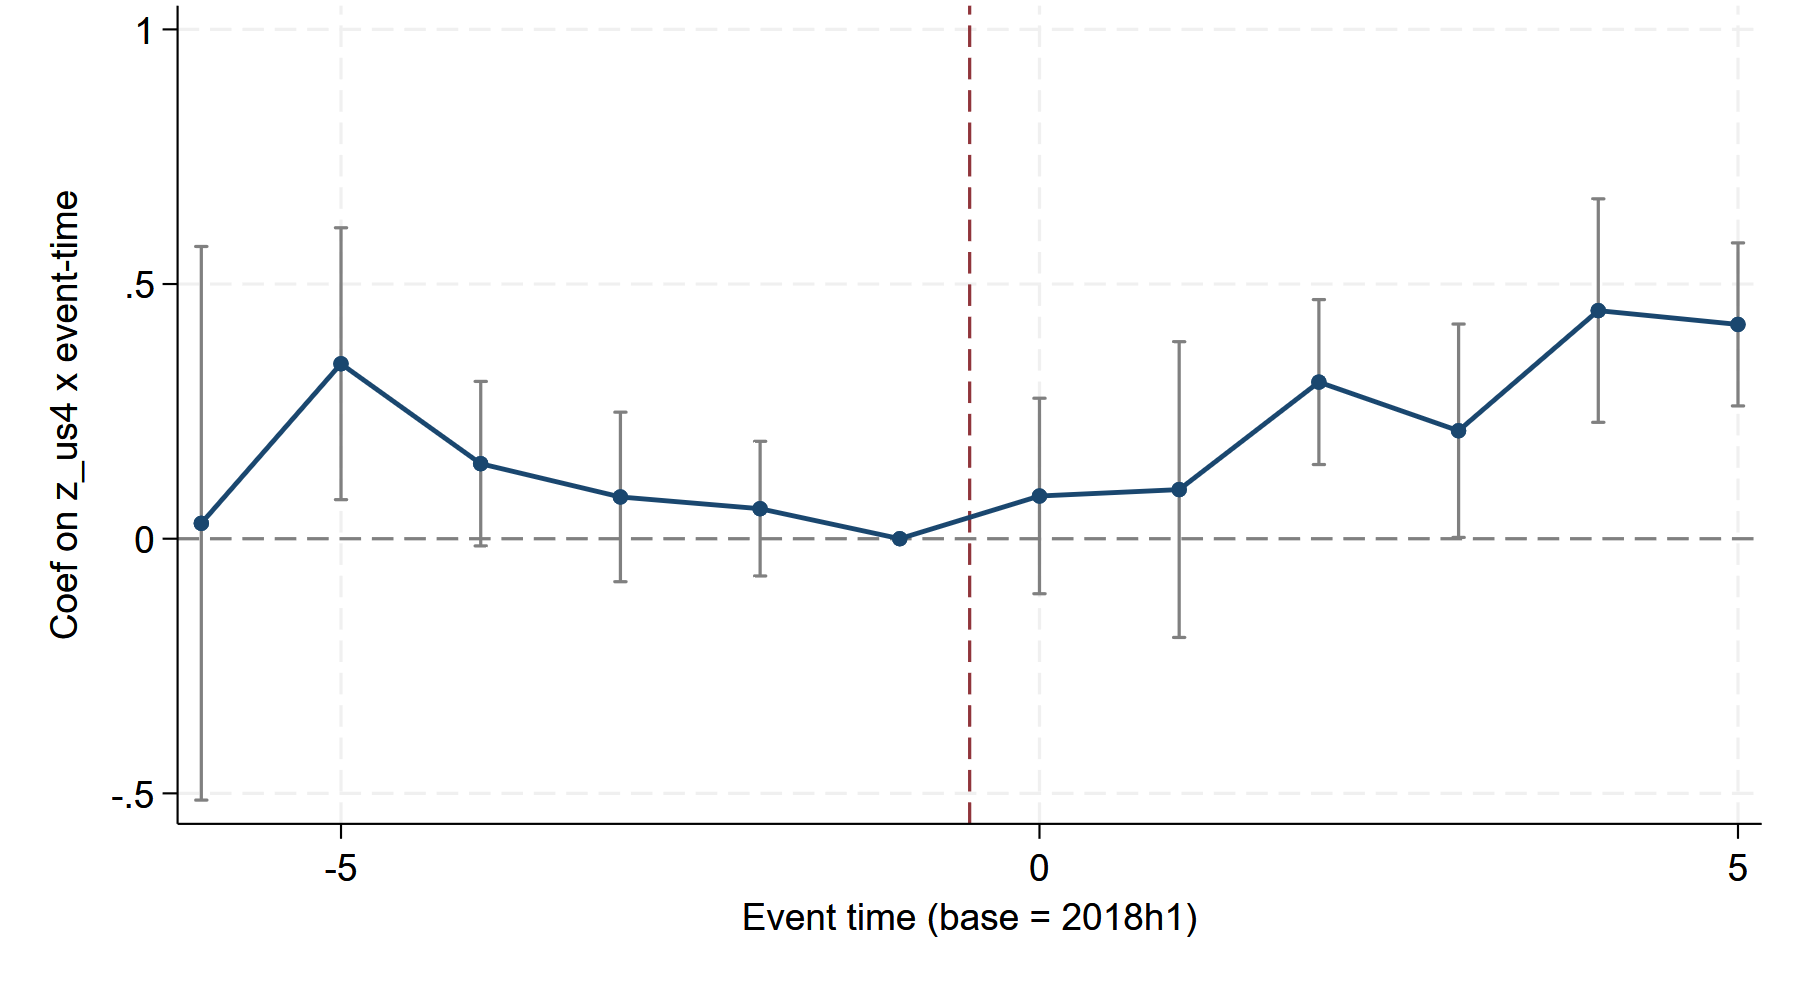
\includegraphics[width=0.68\textwidth]{event_uv_countyfe_100m_v10.png}
  \end{center}
  \vspace{-0.2em}
\end{frame}

\section{空间异质性与分案由讨论}

\begin{frame}[plain]{空间位置异质性：外围城中村更受冲击}
  \centering
  \scriptsize
  \begin{tabular}{lccc}
    \toprule
     & 正规街区 & 中心城中村 & 外围城中村 \\
    \midrule
    $Post\times Exposure$ & 0.093 & 0.177$^{+}$ & 0.158$^{***}$ \\
     & (0.128) & (0.122) & (0.058) \\
    \addlinespace[1pt]
    样本量 & 5,846,172 & 1,197,852 & 674,743 \\
    Pseudo $R^2$ & 0.086 & 0.055 & 0.096 \\
    \bottomrule
  \end{tabular}

  \vspace{0.5em}
  \parbox{0.93\textwidth}{\footnotesize 注：样本为100m网格。$+$表示$p<0.15$；* $p<0.10$，** $p<0.05$，*** $p<0.01$。外围城中村的冲击效应最强。}
\end{frame}

\begin{frame}{犯罪案由异质性：经济压力与灰色空间相关类型更敏感}
  \small 将案由进一步拆分后，冲击并非平均抬升所有犯罪，而是更集中于与\textbf{经济压力、日常摩擦与灰色活动空间}相关的类型。
\end{frame}

\begin{frame}[plain]{案由异质性：16类细分结果}
  \centering
  \scriptsize
  \begin{minipage}[t]{0.48\textwidth}
    \centering
    \textbf{财产型犯罪}
    \vspace{0.25em}
    \begin{tabular}{llcccc}
      \toprule
      16类案由 & 正规街区 & 城中村 & 中心 & 外围 \\
      \midrule
      盗窃 & \makecell{0.117\\(0.152)} & \makecell{0.163*\\(0.086)} & \makecell{0.183\\(0.181)} & \makecell{0.120**\\(0.058)} \\
      诈骗 & \makecell{-0.054\\(0.201)} & \makecell{0.548***\\(0.174)} & \makecell{0.516+\\(0.330)} & \makecell{0.464***\\(0.101)} \\
      抢劫 & \makecell{0.095\\(0.305)} & \makecell{0.062\\(0.230)} & \makecell{-0.511\\(0.363)} & \makecell{0.454***\\(0.114)} \\
      敲诈勒索 & \makecell{0.887+\\(0.569)} & \makecell{0.810*\\(0.418)} & \makecell{-0.420\\(0.912)} & \makecell{6.204\\(4.320)} \\
      \bottomrule
    \end{tabular}
  \end{minipage}
  \hfill
  \begin{minipage}[t]{0.48\textwidth}
    \centering
    \textbf{冲动型犯罪}
    \vspace{0.25em}
    \begin{tabular}{llcccc}
      \toprule
      16类案由 & 正规街区 & 城中村 & 中心 & 外围 \\
      \midrule
      公共安全 & \makecell{0.637\\(0.495)} & \makecell{1.120***\\(0.355)} & \makecell{0.464\\(0.725)} & \makecell{1.866**\\(0.762)} \\
      暴力 & \makecell{0.155\\(0.212)} & \makecell{0.312***\\(0.112)} & \makecell{0.317\\(0.272)} & \makecell{0.298***\\(0.067)} \\
      交通犯罪 & \makecell{-0.260\\(0.372)} & \makecell{0.272**\\(0.130)} & \makecell{0.833*\\(0.434)} & \makecell{0.134+\\(0.093)} \\
      \bottomrule
    \end{tabular}
  \end{minipage}

  \vspace{0.8em}

  \begin{minipage}[t]{0.48\textwidth}
    \centering
    \textbf{企业犯罪}
    \vspace{0.25em}
    \begin{tabular}{llcccc}
      \toprule
      16类案由 & 正规街区 & 城中村 & 中心 & 外围 \\
      \midrule
      知识产权 & \makecell{0.018\\(0.173)} & \makecell{0.464**\\(0.223)} & \makecell{0.481\\(0.431)} & \makecell{0.782*\\(0.457)} \\
      制假售假 & \makecell{0.417\\(0.435)} & \makecell{0.147\\(0.627)} & \makecell{0.157\\(0.599)} & \makecell{3.769\\(11.572)} \\
      贿赂 & \makecell{-0.082\\(0.230)} & \makecell{2.084+\\(1.369)} & \makecell{1.811\\(1.539)} & \makecell{0.626\\(0.700)} \\
      金融 & \makecell{-0.011\\(0.430)} & \makecell{-0.416\\(0.659)} & \makecell{-0.285\\(0.981)} & \makecell{--\\(--)} \\
      \bottomrule
    \end{tabular}
  \end{minipage}
  \hfill
  \begin{minipage}[t]{0.48\textwidth}
    \centering
    \textbf{地下经济犯罪}
    \vspace{0.25em}
    \begin{tabular}{llcccc}
      \toprule
      16类案由 & 正规街区 & 城中村 & 中心 & 外围 \\
      \midrule
      毒品 & \makecell{0.098\\(0.146)} & \makecell{0.183**\\(0.087)} & \makecell{-0.031\\(0.270)} & \makecell{0.196***\\(0.063)} \\
      赌博 & \makecell{0.093\\(0.172)} & \makecell{0.085\\(0.151)} & \makecell{0.035\\(0.307)} & \makecell{0.179\\(0.129)} \\
      淫秽 & \makecell{0.186\\(0.356)} & \makecell{0.188\\(0.167)} & \makecell{0.222+\\(0.153)} & \makecell{0.191\\(1.261)} \\
      走私 & \makecell{1.123***\\(0.077)} & \makecell{-1.677\\(3.698)} & \makecell{-1.759\\(4.441)} & \makecell{--\\(--)} \\
      非法迁徙 & \makecell{-0.134\\(0.579)} & \makecell{--\\(--)} & \makecell{--\\(--)} & \makecell{--\\(--)} \\
      \bottomrule
    \end{tabular}
  \end{minipage}

  \vspace{0.35em}
\end{frame}

\begin{frame}[plain]{案由大类异质性：四类汇总结果}
  \centering
  \scriptsize
  \begin{tabular}{lcccc}
    \toprule
    案由大类 & 正规街区 & 城中村 & 中心城中村 & 外围城中村 \\
    \midrule
    财产型犯罪 & \makecell{0.101\\(0.150)} & \makecell{0.190**\\(0.090)} & \makecell{0.122\\(0.172)} & \makecell{0.190***\\(0.062)} \\
    冲动型犯罪 & \makecell{0.075\\(0.209)} & \makecell{0.320***\\(0.101)} & \makecell{0.344\\(0.247)} & \makecell{0.292***\\(0.061)} \\
    企业犯罪 & \makecell{0.186+\\(0.125)} & \makecell{0.422**\\(0.184)} & \makecell{0.497+\\(0.331)} & \makecell{0.507**\\(0.246)} \\
    地下经济犯罪 & \makecell{0.136\\(0.141)} & \makecell{0.178***\\(0.069)} & \makecell{0.104\\(0.209)} & \makecell{0.201***\\(0.049)} \\
    \bottomrule
  \end{tabular}

  \vspace{0.4em}
    % 注：四大类结果与16类细分方向一致，外围城中村在多类案由上更敏感。
\end{frame}

\begin{frame}[plain]{被告人身份异质性}
  \centering
  \tiny
  \begin{adjustbox}{width=\textwidth}
  \begin{tabular}{lcccccccc}
    \toprule
     & \multicolumn{2}{c}{就业状态} & \multicolumn{2}{c}{性别} & \multicolumn{2}{c}{民族} & \multicolumn{2}{c}{教育} \\
    \cmidrule(lr){2-3}\cmidrule(lr){4-5}\cmidrule(lr){6-7}\cmidrule(lr){8-9}
    案由类别 & 有业 & 无业 & 男性 & 女性 & 汉族 & 少数民族 & 高教育 & 低教育 \\
    \midrule
    总犯罪 & \makecell{0.152***\\(0.036)} & \makecell{-0.126\\(0.219)} & \makecell{0.124***\\(0.040)} & \makecell{0.025\\(0.166)} & \makecell{0.132***\\(0.039)} & \makecell{0.012\\(0.134)} & \makecell{-0.014\\(0.105)} & \makecell{0.138***\\(0.039)} \\
    财产型 & \makecell{0.087\\(0.123)} & \makecell{0.069\\(0.202)} & \makecell{-0.077\\(0.091)} & \makecell{0.079\\(0.179)} & \makecell{-0.682***\\(0.190)} & \makecell{0.152\\(0.172)} & \makecell{0.129**\\(0.051)} & \makecell{-1.051***\\(0.389)} \\
    冲动型 & \makecell{0.466**\\(0.211)} & \makecell{0.041\\(0.194)} & \makecell{0.153**\\(0.063)} & \makecell{0.165\\(0.175)} & \makecell{-0.142\\(0.134)} & \makecell{0.175\\(0.156)} & \makecell{0.178***\\(0.061)} & \makecell{-0.844\\(0.959)} \\
    企业型 & \makecell{0.513***\\(0.106)} & \makecell{-0.135\\(0.367)} & \makecell{0.261\\(0.328)} & \makecell{-0.160\\(0.459)} & \makecell{0.032\\(0.638)} & \makecell{-0.101\\(0.359)} & \makecell{0.208**\\(0.099)} & \makecell{0.706\\(0.739)} \\
    地下经济 & \makecell{0.000\\(0.092)} & \makecell{0.138\\(0.165)} & \makecell{-0.035\\(0.107)} & \makecell{0.112\\(0.198)} & \makecell{-0.641**\\(0.274)} & \makecell{0.168\\(0.140)} & \makecell{0.104***\\(0.040)} & \makecell{-0.423\\(0.291)} \\
    \bottomrule
  \end{tabular}
  \end{adjustbox}

  \vspace{0.35em}
  % 注：表中数值为$Post\times Exposure$的系数。
\end{frame}

\section{补充分析与政策含义}

\begin{frame}[plain]{社会网络的调节效应}
  \centering
  \tiny
  \begin{adjustbox}{width=\textwidth}
  \begin{tabular}{lcccccc}
    \toprule
    \multirow{2}{*}{因变量} & \multicolumn{2}{c}{中心城中村} & \multicolumn{2}{c}{外围城中村} & \multicolumn{2}{c}{全部城中村} \\
    \cmidrule(lr){2-3}\cmidrule(lr){4-5}\cmidrule(lr){6-7}
     & 菜系熵 & 餐馆密度 & 菜系熵 & 餐馆密度 & 菜系熵 & 餐馆密度 \\
    \midrule
    总犯罪 & \makecell{-0.309*\\(0.171)} & \makecell{-0.010\\(0.085)} & \makecell{0.007\\(0.226)} & \makecell{-0.624*\\(0.322)} & \makecell{-0.023\\(0.132)} & \makecell{-0.093\\(0.130)} \\
    财产型犯罪 & \makecell{-0.500**\\(0.205)} & \makecell{-0.080\\(0.233)} & \makecell{0.054\\(0.221)} & \makecell{-0.688+\\(0.429)} & \makecell{-0.001\\(0.209)} & \makecell{-0.065\\(0.096)} \\
    冲动型犯罪 & \makecell{-0.596+\\(0.411)} & \makecell{-0.143\\(0.176)} & \makecell{0.368+\\(0.243)} & \makecell{-1.160**\\(0.486)} & \makecell{0.027\\(0.265)} & \makecell{-0.135\\(0.153)} \\
    企业犯罪 & \makecell{0.037\\(0.279)} & \makecell{-0.767\\(0.570)} & \makecell{0.022\\(0.469)} & \makecell{1.167\\(1.329)} & \makecell{0.099\\(0.125)} & \makecell{-0.411\\(0.454)} \\
    地下经济犯罪 & \makecell{0.026\\(0.164)} & \makecell{0.125\\(0.107)} & \makecell{0.374\\(0.343)} & \makecell{-0.268\\(0.200)} & \makecell{0.182\\(0.202)} & \makecell{0.027\\(0.050)} \\
    \bottomrule
  \end{tabular}
  \end{adjustbox}
  
  \vspace{0.25em}
  \parbox{0.95\textwidth}{\footnotesize 注：表中为三重交互项$Post\times Exposure\times Z$的系数（$Z$为菜系熵或餐馆密度），$Z$已标准化。}
\end{frame}

\begin{frame}[plain,t]{菜系主题词云图}
  \begin{center}
    
\includegraphics[width=0.72\textwidth]{1.描述性证据/lda_topic_wordclouds_multiyear_grid_3x6.png}
  \end{center}
  \vspace{-0.2em}
  \small 该图用于展示餐饮网络与社区社会连接的主题结构。
\end{frame}

\begin{frame}[plain,t]{2017年珠三角菜系熵分布图}
  \begin{center}
    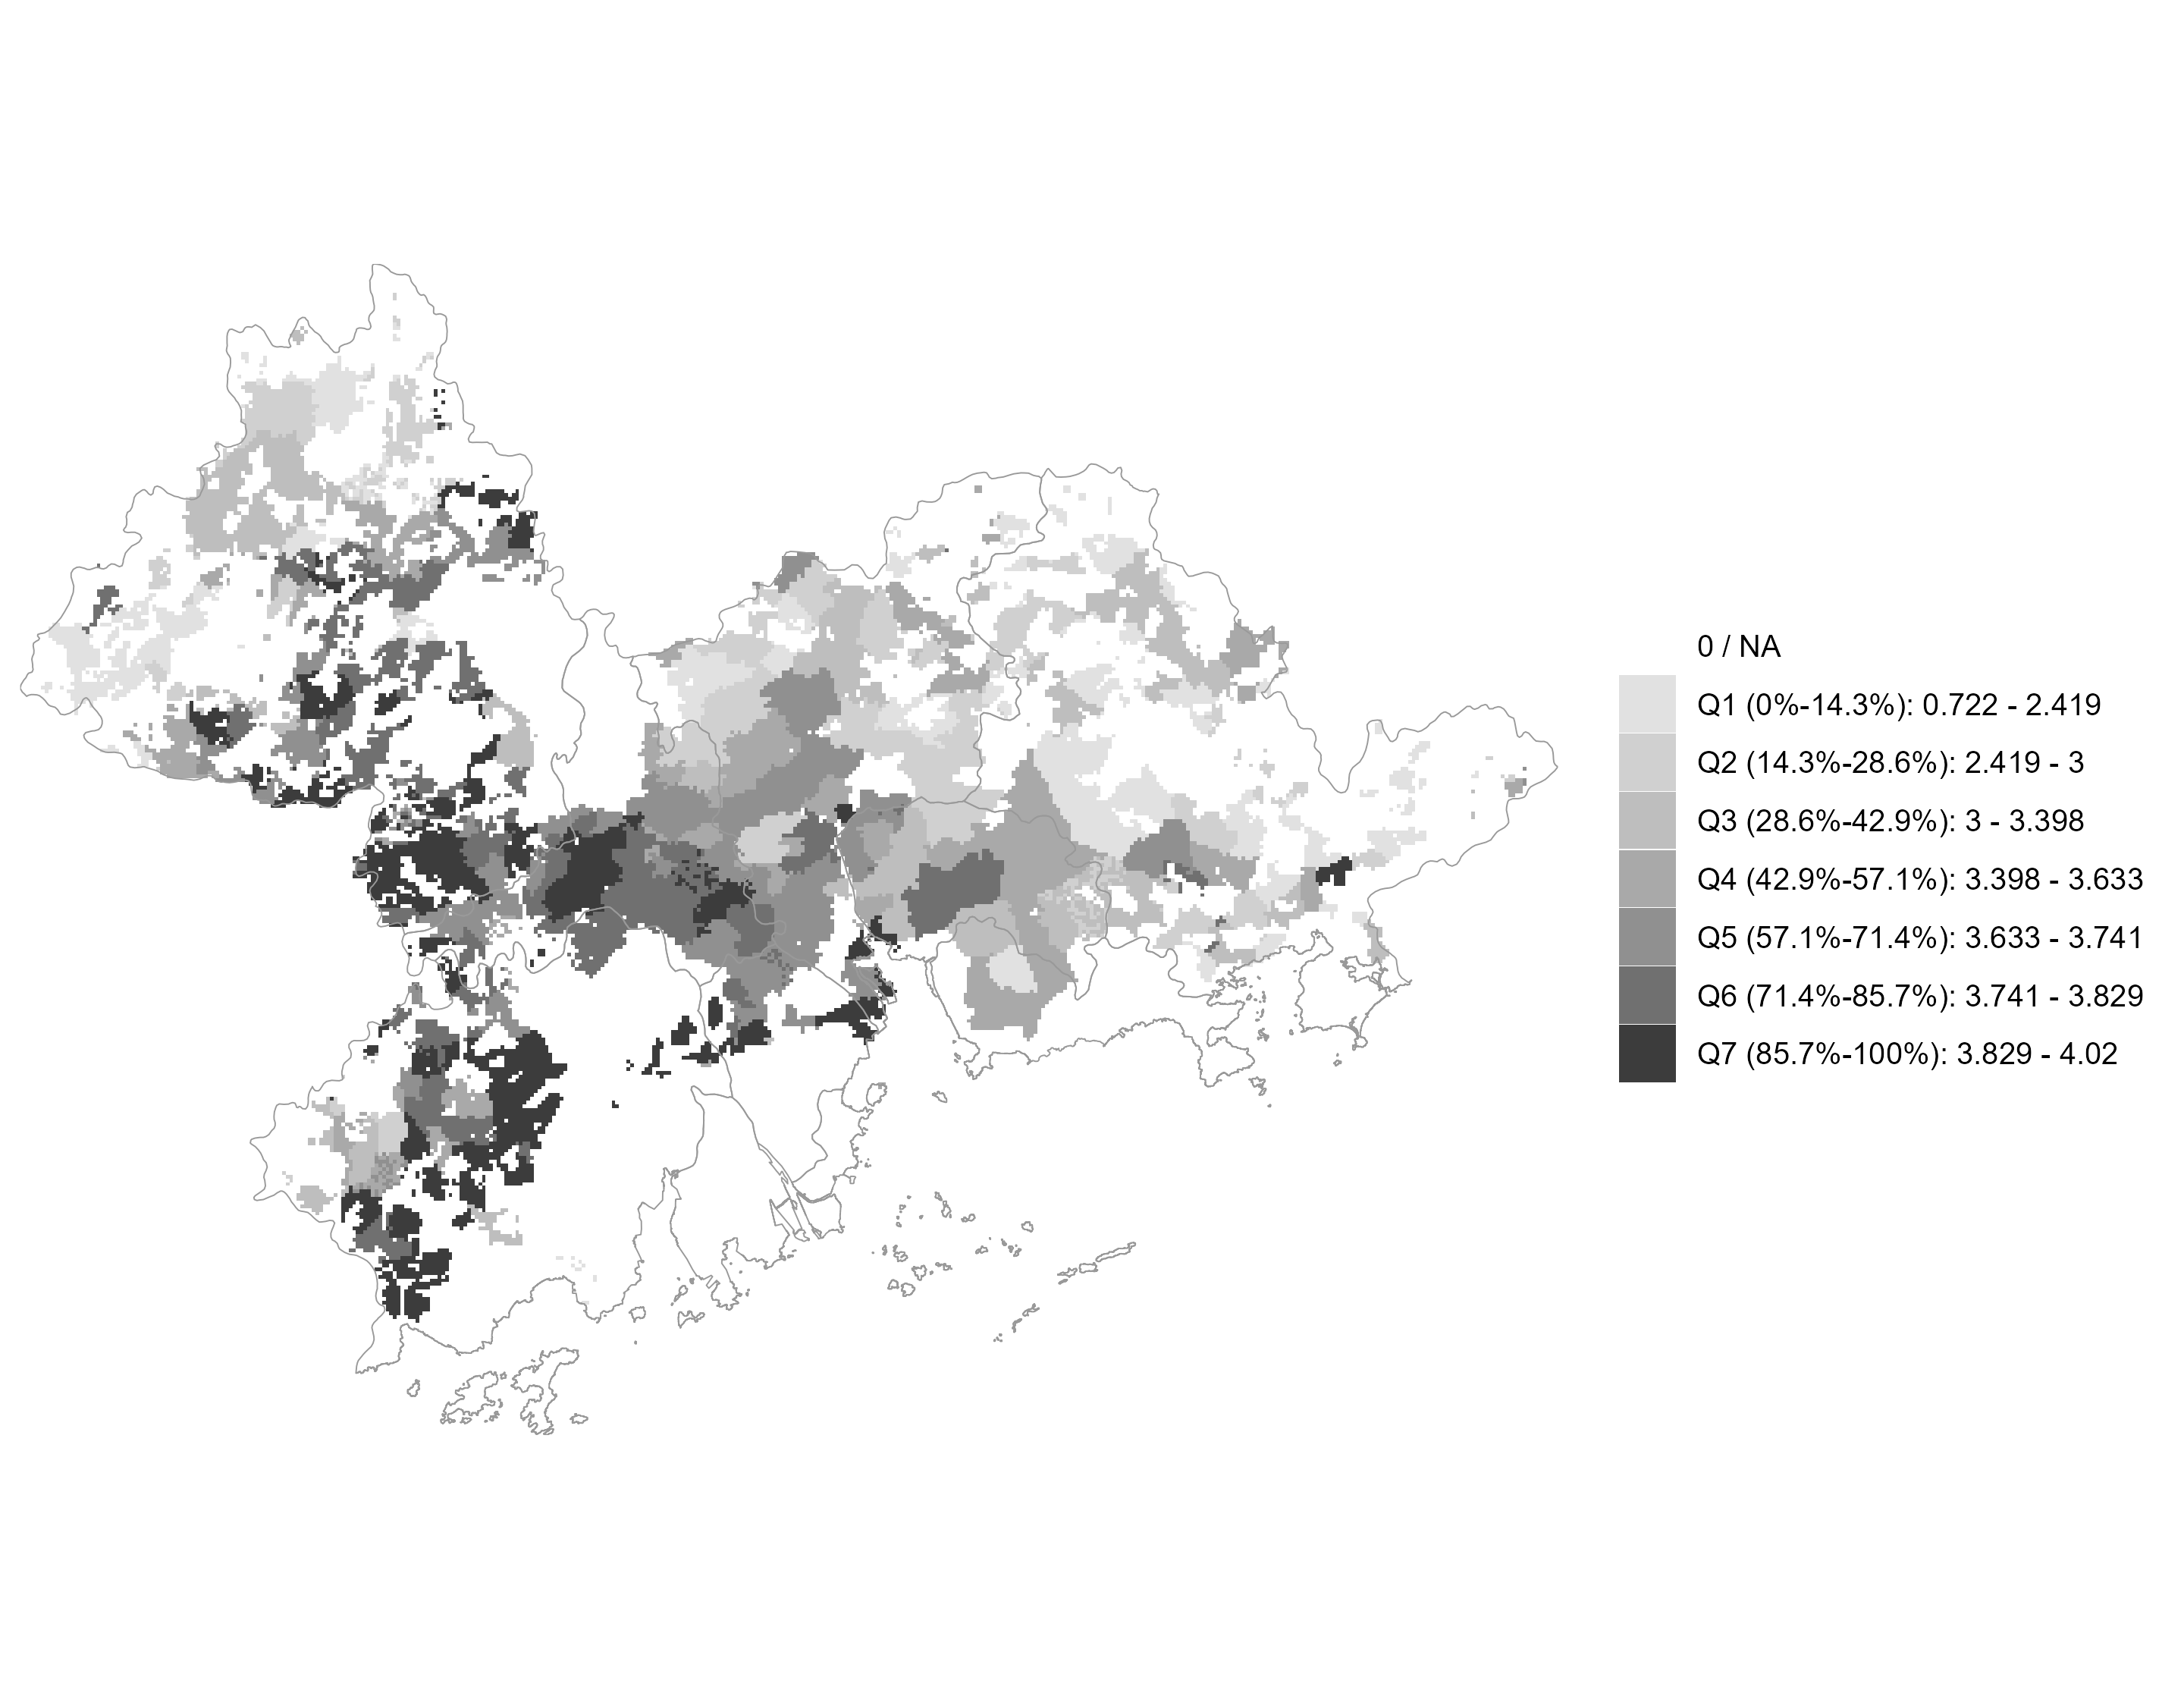
\includegraphics[width=0.72\textwidth]{1.描述性证据/分布图/prd_prefer500m_cuisine_entropy_2017.png}
  \end{center}
  \vspace{-0.2em}
  \small 菜系熵越高，代表餐饮供给越多样化、社区社会连接越复杂。
\end{frame}

\begin{frame}[plain]{关税冲击对二手房、人口与夜间灯光的影响}
  \centering
  \scriptsize
  \begin{minipage}[t]{0.97\textwidth}
    \centering
    \textbf{二手房市场}
    \vspace{0.2em}
    \begin{tabular}{lcccc}
      \toprule
       & 城中村 & 正规街区 & 中心城中村 & 外围城中村 \\
      \midrule
      挂牌单价 & \makecell{-841.300\\(2531.300)} & \makecell{1128.400\\(2183.600)} & \makecell{1285.300\\(2529.500)} & \makecell{-2089.800\\(2161.100)} \\
      成交单价 & \makecell{-1629.200\\(3142.600)} & \makecell{1698.000\\(2072.500)} & \makecell{1207.000\\(2441.300)} & \makecell{-3242.300\\(3088.500)} \\
      议价空间 & \makecell{553.400\\(575.900)} & \makecell{744.800\\(537.400)} & \makecell{1185.500\\(928.400)} & \makecell{85.000\\(346.600)} \\
      成交周期（天） & \makecell{15.360**\\(7.450)} & \makecell{19.090**\\(9.580)} & \makecell{25.170**\\(11.250)} & \makecell{6.000*\\(3.350)} \\
      \bottomrule
    \end{tabular}
  \end{minipage}

  \vspace{0.5em}

  \begin{minipage}[t]{0.48\textwidth}
    \centering
    \textbf{人口}
    \vspace{0.2em}
    \begin{tabular}{lcccc}
      \toprule
       & 城中村 & 正规街区 & 中心城中村 & 外围城中村 \\
      \midrule
      人口对数 & \makecell{0.002\\(0.002)} & \makecell{-0.001\\(0.003)} & \makecell{0.004**\\(0.002)} & \makecell{0.003\\(0.003)} \\
      人口水平 & \makecell{-0.717\\(0.792)} & \makecell{-2.438\\(1.915)} & \makecell{-2.289+\\(1.470)} & \makecell{0.500**\\(0.221)} \\
      \bottomrule
    \end{tabular}
  \end{minipage}
  \hfill
  \begin{minipage}[t]{0.48\textwidth}
    \centering
    \textbf{夜间灯光}
    \vspace{0.2em}
    \resizebox{\linewidth}{!}{%
    \begin{tabular}{lcccc}
      \toprule
       & 城中村 & 正规街区 & 中心城中村 & 外围城中村 \\
      \midrule
      夜间灯光（对数） & \makecell{0.014***\\(0.004)} & \makecell{0.024***\\(0.009)} & \makecell{0.015**\\(0.007)} & \makecell{0.005\\(0.005)} \\
      夜间灯光水平 & \makecell{0.406**\\(0.204)} & \makecell{1.116**\\(0.437)} & \makecell{0.745**\\(0.335)} & \makecell{-0.030\\(0.227)} \\
      \bottomrule
    \end{tabular}
    }
  \end{minipage}
\end{frame}

\begin{frame}[plain]{稳健性：不同暴露度口径与税率设定}
  \centering
  \scriptsize
  \begin{tabular}{lccc}
    \toprule
     & 基准：对美出口暴露度 & 对美出口暴露度 & 全口径出口暴露度 \\
     & （List3=25\%） & （List3=10\%） & （List3=25\%） \\
    \midrule
    $Post\times Exposure$ & 0.188*** & 0.116 & 0.032 \\
     & (0.070) & (0.086) & (0.108) \\
    \addlinespace[1pt]
    样本量 & 1,880,892 & 1,880,892 & 1,880,892 \\
    \bottomrule
  \end{tabular}

  \vspace{0.5em}
  % 注：样本为100m城中村网格。* $p<0.10$，** $p<0.05$，*** $p<0.01$。
\end{frame}

\begin{frame}[plain,t]{稳健性：空间置换检验（Permutation）}
  \begin{center}
    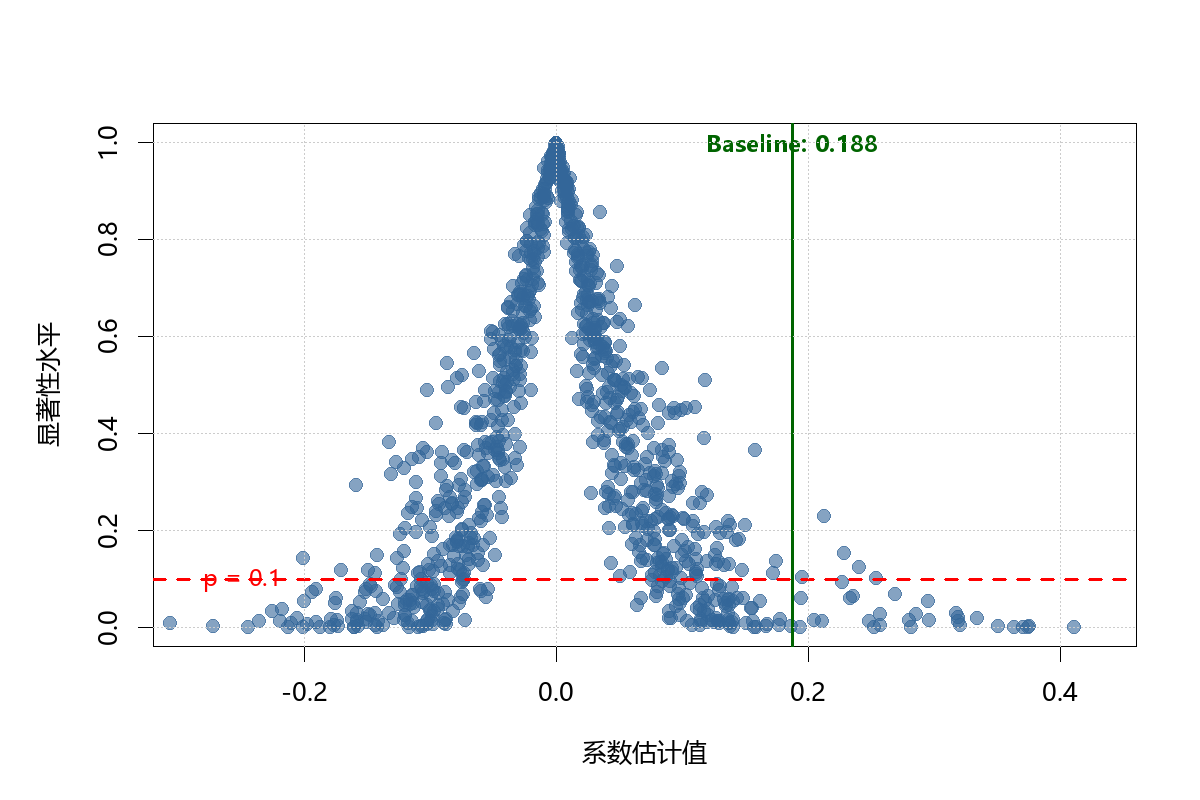
\includegraphics[width=0.70\textwidth]{spatial_permutation_scatter_v1.png}
  \end{center}
  \vspace{-0.2em}
  \small 通过空间置换/随机化思路检验结果不由空间相关性或偶然匹配驱动。
\end{frame}

\begin{frame}{结论与政策含义}
  \begin{enumerate}
    \item 2018年美国关税冲击显著推升珠三角\textbf{城中村}网格犯罪强度（约20.6\%）。
    \item 冲击的治安成本在城市内部\textbf{不均衡}分布：更集中于\textbf{城市外围城中村}。
    \item 风险缓冲：一定的社区社会连接指标对冲击有缓冲迹象。
  \end{enumerate}
  \vspace{0.6em}
  \begin{block}{政策启示}
    在宏观波动期，公共安全与社区治理资源应避免“一刀切”，优先向\textbf{抗压能力更弱的外郊城中村节点}倾斜，并推动民生兜底资源有效下沉。
  \end{block}
\end{frame}

\begin{frame}[plain]
  \begin{center}
    \Large 谢谢！\\[0.8em]
    \normalsize 欢迎提问
  \end{center}
\end{frame}

% =========================
% 附录（备份页）
% =========================
\appendix

\begin{frame}{附录：数据与方法补充（可选备份页）}
  \begin{itemize}
    \item 样本：裁判文书信息抽取与地理编码；案由归并规则；
    \item 网格面板构造：100m基准，稳健性中尝试200m/500m等；
    \item 标准误：按县（区）聚类，允许任意序列/空间相关。
  \end{itemize}
\end{frame}

\section{参考文献}
\begin{frame}[allowframebreaks]{参考文献}
  \scriptsize
  \printbibliography
\end{frame}

\end{document}
